\chapter{Alignments with Pair HMMs}\label{CHAPTER:PAIRHMM}

In this chapter we will describe scoring schemes for pair alignment using pHMMs
or GpHMM. Scoring schemes will differ in two conceptual ways. One way is in the
used model and the second is in the decoding algorithm. At first we show how the
pHMMs can be used to sequence alignment, after that we describe decoding methods
that can be used to reconstruct alignment. The last part of this chapter will
discuss several uses of pHMM and GpHMM to sequence alignment or to the related
problems.

\section{Usage of Pair Hidden Markov Models}\label{SECTION:SIMPLEPHMM}

We can divide states of pHMM into three types.  Ones that generates symbol in
both sequences (match states), states that generates symbol in only one sequence
(indel states) and silent
states. If pHMM generates  symbols in both sequences we consider those symbols
to be homologous. We will consider symbols that were not generated by such state
as indels. Alternative view is to imagine that indel states generate symbol in
one sequence and gap symbol in the second sequence. In such view pHMM generates
an alignment.

Now we show classical pHMM for sequence alignment. It is equivalent to scoring
scheme of Needleman-Wunch algorithm with affine gap model. It consists of three
states: one that generates aligned pairs, and two states for generating
indels (one for each sequence). Model is shown in figure \ref{FIGURE:SIMPLEPHMM}. 

\begin{figure}
\begin{center}
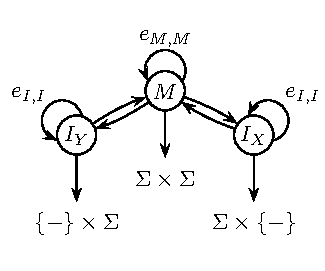
\includegraphics{../figures/pairHMM.pdf}
\end{center}
\caption[Simple pair HMM model for alignment]{Pair hidden Markov model for pair alignment. It has two transitions
parameters $e_{M,M}$ and $e_{I,I}$, since we set $e_{I,M} = 1 - e_{I,I}$ and
$e_{M,I}=\frac12-\frac12e_{M,M}$. Match state $M$ generates aligned pair of symbols
and states $I_X$ and $I_Y$ generates symbols only in $X$ or $Y$ respectively.
Initial distribution is even.
}\label{FIGURE:SIMPLEPHMM}
\end{figure}

As mentioned before, score of the alignment is the probability of state path
that correspond to such alignment. Therefore we can find the alignment with
highest score by two dimensional version of Viterbi algorithm. Advantage of
using this model instead of the Needleman-Wunch algorithm is that pHMM gives
probabilistic explanation of the alignments. 

In following sections we will review several pHMMs and GpHMMs that were used to
sequence alignments or other purpose, for example gene finding. We will review
the application domain of the model, its topology, decoding function, parameter
estimation and optimisation heuristics. But at first, we have to introduce small
biological background.

\todo{zadefinuj quality of an alignment}

\section{Decoding Methods}

In this section we review three decoding methods that were successfully used to
get reconstruct pairwise alignment: the Viterbi algorithm, the Posterior
decoding and the Marginalized posterior decoding.

Let $H$ be an pHMM (or GpHMM) and $X$ and $Y$ be the sequences that we want to
align. The probability $\prob{X,Y\mid H}$ is the probability that $X$ and $Y$
are aligned under model $H$.  From path $\pi$ (or state path and the
sequence of durations in case of GpHMM) we can reconstruct unique alignment.
Such alignment we will denote by $A_{\pi}$.
  \[\prob{\pi\mid
X,Y,H}=\frac{\prob{\pi,X,Y\mid H}}{\prob{X,Y\mid H}}\] is the probability, that
$A_{\pi}$ is alignment of $X$ and $Y$ under the condition, that $X$ and $Y$ were
generated by model $H$.  We can use $\prob{\pi\mid X,Y,H}$ as a score of an
alignment $A_{\pi}$. Such $\pi$ can be found by the two-dimensional Viterbi
algorithm. $A_{\pi}$ can be constructed from $X,Y$ and $\pi$ in straightforward
way: for every match state from $\pi$ (that generated $X[i]$ and $Y[j]$) we add
column $(X[i],Y[j])$. For every indel state in $\pi$ that generates $X[i]$ we
add to alignment column $(X[i],'-')$. Indel state for the second sequences are
analogous.  The two-dimensional Viterbi algorithm is used in the most of the
applications we will discuss later.

Now we show two variants of the Posterior decoding for the pHMMs (the Posterior
decoding and the Marginal posterior decoding).  Let $\prob{X[i]\sim Y[j]\mid
X,Y,H}$ be the probability that $X[i]$ and $Y[i]$ are aligned (sum of the
probabilities of all alignments which contains column $(X[i],Y[i])$. Let
$\prob{X[i]\sim -_j\mid X,Y,H}$ be the probability that $X[i]$ is aligned to a
gap that is in $Y$ between positions $j$ and $j+1$ and let $\prob{-_i\sim
Y[j]\mid X,Y,H}$ be the probability that $Y[j]$ aligned to gap in $X$ between
positions $i$ and $i+1$.  Similarly, let $\prob{X[i]\sim - \mid X,Y,H}$ be the
probability that $X[i]$ is aligned to a gap at any position and let $\prob{-\sim
Y[j]\mid X,Y,H}$ be the probability that $Y[j]$ is aligned to a gap at any
position.  Posterior probabilities defined above can be computed by the
two-dimensional version of the Forward-Backward algorithm (probability that
symbol is aligned to any position is the sum of the probabilities that symbol is
aligned to a gap at position $i$ for all possible positions $i$).

Let alignment $A$ of an sequences $X$ and $Y$ has length $n$ and
consists from columns $a_0,a_1,\dots a_{n-1}$. Each column $a_i$ is pair
$a_i=(x_i,y_i)$ where $x$ and $y$ is either symbol from $\Sigma$ or a gap
symbol\footnote{Note that $x$ and $y$ can't be both gap symbols.}.
Let $d_A^x(i)$ be the number of non-gap symbols in $x_0,x_1,\dots x_i$
and $d_A^y(i)$ be the number of non-gap symbols in $y_0,y_1,\dots, y_i$ and
$d_A^x(-1)=d_A^y(-1)=0$. Intuitively, $A[0:i]$ is alignment of $X[:d_A^x(i)]$ 
and $Y[:d_A^y(i)]$. Then the posterior probability of an alignment column is
\[P(a_i)=
\begin{cases}
\prob{X[d_A^x(i)-1]\sim Y[d_A^y(i)-1]\mid X,Y,H} & \text{if $x_i$ and $y_i$ are not gap symbols}\\
\prob{X[d_A^y(i)-1]\sim -_{d_A^y(i)-1}\mid X,Y,H}  & \text{if $y_i$ is gap symbol and $x_i$ not}\\
\prob{-_{d_A^y(i)-1}\sim Y[d_A^y(i)-1]\mid X,Y,H}  & \text{if $x_i$ is gap symbol and $y_i$ not}
\end{cases}
\]

The \abbreviation{Posterior decoding}{PD} find the alignment $A=a_0a_1\dots
a_{n-1}$ that maximizes
the product of the posterior probabilities of it's columns: 
\[A = \arg\max_{A'\in Al(X,Y)}\prod_{0\leq i <
|A'|}P(a'_i)\] where $Al(X,Y)$ denote the set of all  alignments of a sequences
$X$ and $Y$. Similarly we can define \abbreviation{Marginalized posterior
decoding}{MPD}: Let $P'(a_i)$ is the marginalized posterior probability:
\[
P'(a_i) = \begin{cases}
P(a_i) & \text{if $x_i$ and $y_i$ are not gap symbols}\\
\sum_{0\leq j < |Y|}\prob{X[d_A^y(i)-1]\sim -_{j}\mid X,Y,H}  & \text{if $y_i$ is gap symbol and $x_i$ not}\\
\sum_{0\leq j < |X|} \prob{-_{j}\sim Y[d_A^y(i)-1]\mid X,Y,H}  & \text{if $x_i$ is gap symbol and $y_i$ not}
\end{cases}
\]
Then the MPD find alignment $A=a_0a_1\dots a_{n-1}$ that maximizes
\[A = \arg\max_{A\in Al(X,Y)}\prod_{0\leq i < |A'|)}P'(a'_i)\] 
where $A'=a_0a_1\dots a_{k}$ for some $k$.

The Posterior decoding and the Marginalized posterior decoding were used by
Lunter {\it et al.} and both produced better alignments then alignments founded
by the Viterbi algorithm (the measure in which those alignments were better will
be described later). Once posterior probabilities of all possible columns of an
alignments are computed, we can found the alignment that maximized the desired
function in $O(|X||Y|)$ time \cite{Lunter2008}. 

%Other decoding method can be done by the poster
%Other option is to
%use the  Posterior decoding: for every pairs of residues $X[i],Y[j]$ we compute
%posterior probability that $X[i]$ and $Y[j]$ are aligned $\prob{X[i]\sim Y[j]\mid X,Y,H}$.
%Score of an alignment is sum of posterior probabilities of the aligned residues.
%Later in this chapter we show different variants of the Posterior decoding for
%pHMM.


\section{Pair Hidden Markov Models And Gene Model}

In this section we describe several pair hidden Markov models (or generalized
pair hidden Markov models) with gene structures incorporated into their
topology. These models were used either to alignment of coding DNA or proteins
to genome or to the comparative gene finding.

TODO: Tu bude mega obrazok (asi na jednu stranu), kde budu nakreslene rozne
topologie.

%\subsection{Genes}

%Gene, codon, exon, intron, triplets,..., evolution rate, splice site

At first we introduce several comparative gene finders. Comparative gene finders
use evidence from two organism to find genes. They use pHMM to simultaneously  
align and annotate sequences. 

\subsection{DoubleScan}
Meyer {\it et al. (2002)} developed comparative gene DoubleScan.
Generally, DoubleScan has three types of
states: {\it match} states, which generated same number of symbols in both
sequences;   {\it emit} states, which generate sequences only in one sequence
and silent states. DoubleScan's HMM contains structures for exons, introns and
intron-like structures that are outside genes. 

Basic structure of GpHMM consists from three types of substructures:
substructures that emits exons, substructure that emits introns and substructure
that generates intergenic regions. Each structure was in the alignment three
times: once from match states and twice as emit states. Exon substructure was
single state emitting codons (triplets that will be translated into proteins).
There was one additional intron substructure that was connected to states that
generated intergenic regions. This additional intron substructure was in the
model to avoid detecting of pseudogenes. This GpHMM has $54$ states.

%Every such
%structure has three version: one matching version, which emit aligned residues
%and one structure per sequence to emit indels.  Overview of DoubleScan's HMM
%structure is in figure \ref{}. 
\nocite{Meyer2002}

Emission probabilities if the {\it match exon} state were estimated from
relative frequencies in the training set with Dirichlet priors
\cite{Meyer2002,Durbin1998}.  Emission probabilities of other states were
generated  by marginalizing emissions of the match exon state. Transition
probabilities from initial state were even, transition probabilities for splice
sites were estimated by splice site predictor. Other transitions were observed
from train data and tuned by hand.

DoubleScan uses Viterbi algorithm as decoding method.  To reduce running time of
Viterbi algorithm they use stepping stone algorithm: at first they run BLASTN to
find local alignments. Then DoubleScan choose consistent subset of matching by
greedy method described in section \ref{SECTION:SSA}. They restrict Viterbi
algorithm to such subset allowing tolerance 15 bases.

\subsection{SLAM} 

SLAM \cite{SLAM2003}  is comparative gene finder based on generalized pair
hidden Markov model \cite{Alexanderson2004} with some states being also a
high-order states (with dependence on previous emissions).  It predicts gene
structures for pair of related eukaryotic organisms. SLAM's decoding method is
Viterbi algorithm. 

Unlike DoubleScan, SLAM defines true GpHMM because state durations are not
constant, but are sampled from some distribution (however, distribution they
used in not specified). Topology of the model can be found in figure
\ref{FIGURE:SLAM}.
Emission of pairs of codons were assigned from codon-based PAM matrix.

\begin{figure}
\begin{center}
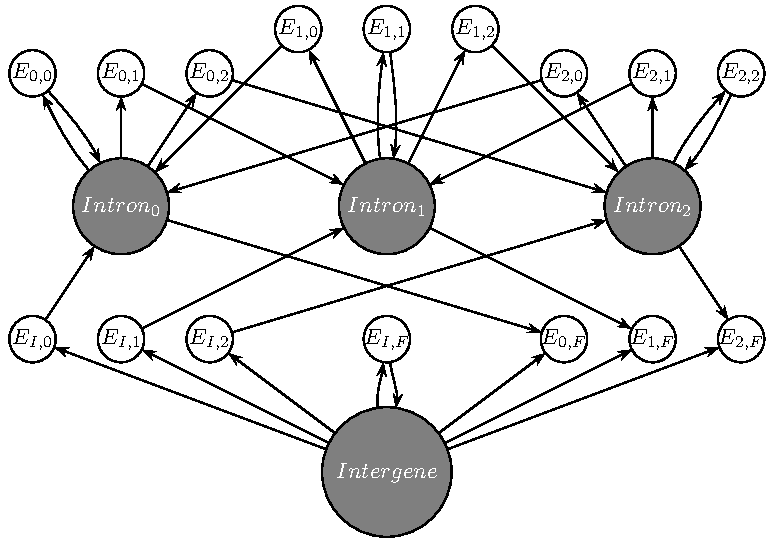
\includegraphics{../figures/slam.pdf}
\end{center}
\caption[HMM topology of SLAM's GpHMM]{
Topology of GpHMM used by slam (states for genes on reverse strand are omitted).
Gray states has geometric distribution (modeled with self-loop which are omitted
in the figure). Emissions of shaded states are done with three state pHMM. White
states econdes exons. Each has associated duration distribution and emmisions
are done also with three-state pHMM ($5$-th order that emitted codons at once).
Since introns can be inside codon model contain exon state for every possible
interruption: $E_{i,j},0\leq i,j<3$ is exon that begin with end of the prevous
exon of length $((3-i)\mod 3)$ and end with the beginning of the exon with
length $j$. $I$ stands for start codon and $F$ stand for stop codon: states
$E_{I,\cdot},E_{\cdot,F}$ and $E_{I,F}$ models exons adjecent to the begininning
and the end of a gene.  $Intron_i$ models intron that interrupted codon on
$i$-th position ($0$ means that intron is not interrupting any codon).
}\label{FIGURE:SLAM} \end{figure}

To reduce running time of the algorithm, they restrict the computation of
alignment in following way: At first they  align input sequences using AVID
alignment tool\cite{Bray2003} to get anchor alignment. They restrict the Viterbi
algorithm in such way, that it could align  in a way, that every base from
bases were extended to intervals of size $3$ bases of bases surrounding each
matching base.



\subsection{Twain}

Twain is another approach to use GpHMM (and evidence from two related genomes)
to find genes \cite{Majoros2005}. It uses interesting technique to improve
running time of the algorithm. It search in the both sequences for the signals
(like ...,..,..,). After that it creates graph: two signals in one sequence are
connected by an oriented edge if one signal can follow other signal. They do
Cartesian product of such graph of both sequences. Resulting graph is used to
restrict search space of the sequence alignment.



\subsection{GeneWise}

GeneWise is protein (or profile HMM) to DNA aligner \cite{GeneWise2004}. It aligns
proteins to homologous exons in DNA. Instead of pHMM defined as in chapter
\ref{}, it used probabilistic transducers (which are similar to pHMM). Main
difference in their model was that emissions were defined for transitions and
not for states.  It's model was created by combining of the gene prediction
model (model $S$) and protein homology model (model $T$). Both models were
represented as pHMM or \correction{transducers}{Napis co to je v kapitole o
HMM}. While model $S$ translates DNA into protein sequence, $T$ was simple pHMM
from section \ref{SECTION:SIMPLEPHMM} defined over protein alphabet
(technically, $T$ translates one protein to another homologous protein).
Combined model was created by composition of models $T$ and $S$, from which were
removed unnecessary states. To decrease state space even more, they remove more
states, for example poly-pyrimidine states. More details are in
\cite{GeneWise2004}.

Parameters for match and insert transitions were derived from amino acid
distribution from the model $T$, from the codon bias in the organism and there
was allowed one substitution error while translating codons to amino acids (due
sequencing errors).
  
\subsection{Pairagon}

Pairagon alignes \abbreviation{coding DNA}{cDNA} to  genome \cite{Pairagon2009}.
To do this task, Pairagon's HMM models consists from simple pair HMM submodel,
which aligns cDNA to DNA and 5 state submodel for intron structures (donor site,
intron, branch, branch acceptor and acceptor state). This model includes 8 base
\abbreviation{weighted matrix model}{WMM} at donor site and 6 base WMM at
acceptor size. Whole topology is in figure \ref{}.

Model was trained using iterative maximum likelihood approach. At first they
trained almost all parameters on BLAT alignments from the
\abbreviation{Mammalian Gene Collection}{MGC}. In this phase, probabilities of
canonical intron, the branch point and the sequence models were set by hand.
After that they used estimated parameters to align more MGC sequences, from
which were the rest of the parameters estimated.

Decoding was done by Viterbi algorithm. Runtime of the algorithm was improved by
stepping stone algorithm \cite{} and memory requirements were improved using
Treeterbi algorithm. 

\section{Aligning Using Different Rates of Evolution}
 
%\subsection{FEAST} 
FEAST is pairwise local alignment tool \cite{FEAST2011}. Simple pHMM from figure
\ref{FIGURE:SIMPLEPHMM} is optimized for one fixed rate of evolution. However,
in DNA conservation rate is different on different sites.  FEAST contain $k$
such submodels, each trained for different rate of evolution. Submodels are
connected with single silent state. Since FEAST is local alignment tool, it one
additional submodel for generating unaligned pair of the sequences 

To construct alignment (either local or global) FEAST uses the Viterbi
algorithm. Like many local aligners, FEAST use seeding heuristics to reduce
computational complexity of finding local alignments.  At first it use six
different space seeds to get candidate seed and extended those seeds using
x-drop heuristic \cite{} using ungapped version of Forward algorithm during
extension (Viterbi algorithm is usually used during extension phase).

Estimation of parameters was done by expectation maximization approach (with
Baum-Welch or Viterbi training). They forced gap parameters to be same in all
submodels.

Using different rate of evolution was also used in \cite{NovyLunter}. Such HMM
contained several states for the most probable alignemnt

Dalsie modely: TWINSCAN, MCALIGN2, WABA, Catwright (zeta function)

\section{Non-Geometric Indel Models}
\todo{Povedat niekde ze preco je afiinne rozdelenie geometricke}
In simple pHMM described in figure \ref{SECTION:SIMPLEPHMM}, gap's length have
geometric distribution: the probability that gap have length $n$ is
$e_{M,I}e_{I,I}^{n-1}(1-e_{I,I})$ (if we sum out all emissions).  Viterbi
algorithm is usually computed in log-space: instead of computing product of
probabilities of events\footnote{Event is emission or transition.}, we compute
the sum of logarithms of those probabilities, because computation in log-space
is numerically more stable. Viterbi algorithm for the simple HMM
will became same as the Needleman-Wunsch algorithm.  Gap penalty will be
$\log(e_{M,I})+\log(1-e_{I,I})+(n-1)\log(e_{I,I})$. By setting $d=\log(e_{I,I})$
and $g=\log(e_{M,I})+\log(1-e_{I,I})-d$ we see that this is exactly affine gap
penalty. Therefore we can say that affine gap penalties corresponds to geometric
distribution of indel lengths.

As we mentioned chapter \ref{CHAPTER:ALIGNMENT}, using non-affine gap model can
improve alignment quality.  Problem with geometric distribution (or affine gap
penalties) is that it gave too high penalty for long indels \cite{} Therefore
some other distribution might be more appropriate, for example zeta distribution
\cite{}, or combination of several geometric distributions to approximate final
distribution \cite{}.

GpHMM are suited to usage of different then geometric duration distributions.
On the other hand, GpHMM are slower to decode so we might want to avoid them if
possible.  One way of incorporating different gap distribution into pair hidden
Markov models without using theirs generalized version is to use several (for
example two) indel states for every sequence. For example FASTA \cite{} and
Lunter {\it et al. (2008)} used two component mixture models: instead of one
indel state for every sequence we use two indel states for every sequence. They
report that this improved quality of alignments.

Modeling non-geometric distributions with several states can be problematic. Set
of states with same emission distribution used for modeling modeling
non-geometric distribution is called gadget (There are also additional
properties: all transitions entering gadget has to either start in same state or
end in same state. Same holds for transitions that leaves gadget. ). Problems
with gadgets and the Viterbi algorithm are discussed in
\cite{TomasovaDizertacka}. We describe discuss those problems for the two
component mixture models.

Let $H$ be an simple pair hidden Markov model with two pairs of indel states.
Let $I_1$ and $I_2$ be indel states that generates gaps in the first sequence.
Gaps in alignments (in the first sequence) that are generated by such model has
distribution $d(n)=(a_1p_1^n(1-p_1)+a_2^n(1-p_2)), n>0, d(0)=1-a_1-a_2$ where
$n$ is the length of the gap, $a_1$ and $a_2$ are probabilities of entering
state $I_1$ and $I_2$ respectively and $p_1$ and $p_2$ are probabilities of
remaining in state $I_1$ and $I_2$ respectively. This is equivalent to
generalized pair hidden Markov model $H'$ with one indel state for every
sequence which have $d(n)$ as it's duration distribution. Both models defines
same distributions of alignments (but not distribution of alignments and state
paths) and running the Forward-Backward algorithm or the Forward algorithm will 
give same results. However, alignments constructed by the Viterbi algorithm
might be different for $H$ and $H'$.

Problem is that in the generalized model the Viterbi algorithm gaps of length
$n$ have ``score'' $d(n)$ but in the non-generalized pair hidden Markov model it
will be $m(n)=\max\{a_1p_1^n(1-p_1),a_2p_2^n(1-p_2)\}, n>0$ and
$m(0)=1-a_1-a_2$.  These two scores are different ($d(n)$ is always higher) and
therefore it is possible that the Viterbi algorithm reconstruct different
alignments. Therefore if we are using the Viterbi algorithm we should either
train such gadget that $m(n)$ will be better approximation of $d(n)$ of the
original model or to use generalized pair hidden Markov model for the Viterbi
algorithm or some variant of the most probable state path.


%co chcem povedat: niekedy je lepsie pouzit iny gapmodel -- jeden pre kratke
%gapy, jeden pre slhe gapy. Preto sa niekedy 


\section{Biases In Alignments}

Lunter {\it et al. (2008)} conducted extensive survey concerning biases in
alignment. They considered three types of biases (associated with gaps). These
gap biases are also discussed in \cite{Durbin1998} \todo{Naozaj?}. By
\firstUseOf{true alignment} we mean alignment that corresponds to actual 
evolution history.
\begin{itemize}
\item \firstUseOf{Gap wander} means that gap is in different location that in
true alignment. Is is due to random short similarities around the borders of
a gaps that are indistinquishable from true homologies. Lunter {\it et al.} gave
explicit formula for computing the expected proportion of incorrectly aligned
regions due to gap wander. \todo{Nie je tento vzorec zbytocny?}
\[F_w =
\frac{\sigma}{\gamma}\frac{(4e^{4\sigma/3}-3)(4e^{\sigma/3}-1)}{8e^{4\sigma/3}-3}\]
where $\gamma$ is th ratio of the substitution rate, $\sigma$, to the indel
rate, $\sigma$.

\item \firstUseOf{Gap attraction} is caused when two gaps are near each other.
In such case merging those caps and introducing few mismatches might have higher
score. 
\item \firstUseOf{Gap anihilation} occurs when there are two gaps with
same length in both sequences. Since indels are not so common, removing both
gaps while introducing new mismatches might increase score of an alignment.
\end{itemize}

Biases are ordered by their frequency from the most occurring to the least
occurring \cite{Lunter2008}. They did a simulation study: they simulate
evolution the human and mouse sequence to get sequences with true alignments.
After that they align those sequences using several pHMMs with several decoding
algorithm; from the simple pair hidden Markov model from figure
\ref{FIGURE:PAIRHMM} to the pHMM with two component geometric mixture models and
variable evolution rate depending on GC content. They used three decoding
algorithm: The Viterbi algorithm, the Posterior decoding and the
\abbreviation{Marginalized posterior decoding}{MPD}.

%Let $X$ and $Y$ be input sequences and $H$ be an pHMM. Let $M_{i,j}$ be the
%probability that $X[i]$ and $Y[j]$ are aligned (this corresponds to column
%$(X[i],Y[j])$ in the alignment), $M^X_{i,j}$ be the probability that $X[i]$ is
%aligned to a gap between positions $j$ and $j+1$ in a sequence $Y$ (this
%corresponds to column $(X[i],'-')$ in the alignment) and $M^Y_{i,j}$ be the
%probability that $Y[j]$ is align to a gap between position $i$ and $i+1$ in a
%sequence $X$ (column $('-',Y[j])$ of an alignment). The values $M_{i,j}$,
%$M^X_{i,j}$ and $M^Y_{i,j}$ defines posterior probabilities of all possible
%columns in alignment. Their Posterior algorithm maximizes the sum of logarithms
%of the probabilities of all column in alignments (or the product of their
%probabilities). The MPD differs in the treatment of gaps. Gap probabilities does
%not depend on position. $M^X_{i,j}$ is defined as the probability that $X[i]$ is
%aligned to a gap (at any position) and $M^Y_{i,j}$ is analogous.
%%= \sum_{k}M^X_{i,k}$ and
%%$M^Y'_{i,j}=\sum_{k}M^Y_{k,j}$.
%
%PD and MPD created alignments with higher sensitivity and  false-positive ratio
%independently of the used model.  Usage of mixtu

Their study shows that 
